\chapter{Appendix for Chapter 3}

\section{Comments on specific objects}\label{apdx:comments}
%####################################################################
% \subsection{WR 4}

\textbf{WR 4:} According to the seventh catalogue of WR stars \citep{2001vanderHucht}, WR 4 is classified as a WC5+?, an SB1 with no observable line dilution or absorption effects. Photometric variability with a period of 4.3 days \citep{1986MoffatShara} was determined. \citet{1989RustamovCherepashchuk} found both a photometric and spectroscopic period of 2.4096 days with a peak-to-peak amplitude of ${\sim}$60\kms, but we can safely reject the presence of such large amplitude RV variation in our data set (Table \ref{tab:WC_data}) questioning the fact that the 2.4~d period traces  an orbital motion. We therefore do not include WR 4 in the list of short-period binaries in our literature study (Sect. \ref{subsec:GWC_bin}).

In a study of co-rotating interaction regions (CIRs), \citet{2009StLouis} classified WR 4 as `Not Variable' in the weak C {\sc iv} 5016\,\r{A} line. \citet{2011CheneStLouis} further elaborated that the maximum line-profile variability was 1.2\% of the level of flux in the line, hence making it ineligible to be a CIR candidate. In this work, we obtained 22 epochs over a time coverage of 890 days, out of which about 12 were observed within two nights, attempting a probe on shorter periods. Although we do not report a short period, the adopted choice of our threshold allows us to classify it as a binary (Table \ref{tab:WC_data}). Further monitoring of this system is required to determine the orbital period of this system.

% \subsection{WR 5}

\textbf{WR 5:} \citet{2001vanderHucht} reports WR 5 as a single star with spectral type of WC6. No emission was found in the X-rays \citep{Skinner2006,2009GudelNaze}. In this work, WR 5 is found to have a \DelRV{} of 4.9\,\kms{} over 718 days with a $\sigma_\textrm{RV}$ of 1.7\,\kms{} for RVs measured using the full spectrum. It does not pass our binary detection criterion and is, therefore, classified as presumably single.

% \subsection{WR 111}

\textbf{WR 111:} WR 111 is a presumably single WC5 star \citep{1999aNiemela,2001vanderHucht}. It has been studied with spectral analyses and hydrodynamical studies \citep{2002Grafener,2005GrafenerHamann,2012Sander}, and was used to show for the first time that WC winds can be explained through radiation-driven mass loss. In this work, WR 111 shows a peak-to-peak variability of 4.5\,\kms{} over 742 days with a $\sigma_\textrm{RV}$ of 1.5\,\kms{}. It does not pass our binary detection criterion and is therefore classified as a presumably single star.

% \subsection{WR 113}

\textbf{WR 113:} WR 113 is a WC8d+O8-9 binary system first identified by \citet{1981MasseyNiemela} with a period of about 29.707 days in a circular orbit. A debate about the eccentricity arose when \citet{1996Niemela} derived similar orbital parameters with a significant eccentricity ($e=0.19$). The matter was resolved by \citet{2012David-Uraz}, who showed that the two were indistinguishable solutions and adopted a circular orbit and was later confirmed by \citet{2018Hill} with a period of 29.700 $\pm$ 0.001 d. In this work, WR 113 has the largest \DelRV{} and $\sigma_\textrm{RV}$ of 282.6 and 93.9\,\kms{} respectively, passing our binary detection criterion. The RV measurements phased with the orbital period are shown in Fig. \ref{fig:known_orbits}. 

% \subsection{WR 117}

\textbf{WR 117:} According to the GCWR, WR 117 is classified as a WC9d, which is a dust producing star. \citet{2012Sander} find it to be a bit too hotter than most WC9 counterparts, even suggesting it might be in the WC8 parameter regime. \citet{2005Williams} did not find any evidence for an OB-type companion, and hypothesize that WR 117 might be an evolved WC9 star. A large scatter in photometric magnitudes was observed by \citet{2014Williams} with possible 0.5 mag eclipses due to dust. In this work, WR 117 shows a \DelRV{} of 4.9\,\kms{} and a $\sigma_\textrm{RV}$ of 1.9\,\kms{} over a coverage of 488 days and is hence classified as a presumably single star.

% \subsection{WR 119}
\textbf{WR 119:} WR 119 is classified as a single WC9d star according to the GCWR. \citet{2009Fahed} studied it using $V$ and $I$ band photometry, finding a larger than normal variability in these bands. \citet{2017Desforges} performed a temporal variance spectrum analysis over timescales of days to weeks and found significant variability in the  C {\sc iii} 5696\,\r{A} line. In this work, we find values of \DelRV{} and $\sigma_\textrm{RV}$ of 11.0 and 3.2\,\kms{} respectively, resulting in WR 119 being classified as a binary. 
% The RV plot over time can be seen in Appendix 3? \textbf{(tbm)}. Whether this variability is intrinsic or due to orbital motion is a question that will require more observations to answer.

% \subsection{WR 135}

\textbf{WR 135:} WR 135 is an apparently single WC8 star (GCWR). Previous RV studies have failed to determine any variability \citep{1999aNiemela}, nor even photometric variability \citep{1986MoffatShara}. In this work, we find a \DelRV{} of 4.7\,\kms{} and $\sigma_\textrm{RV}$ of 1.6\,\kms{} over a baseline of 2660 days, classifying it as a presumably single star.

% \subsection{WR 137}
\textbf{WR 137:} WR 137 is a well-studied, long-period binary system with a late-type WC star and a late-type O star (WC7pd + O9 V; p: peculiar, d: dust producing). \citet{1999MarchenkoDust} reported dust production in 1997 September - 1998 May and \citet{2001WilliamsDust} derived a period of 13.05 $\pm$ 0.15 years by tracking the periodic dust formation. This period was verified by the orbital analysis using RVs by \citet{2005Lefevre}, who found the maximum emission from dust to occur just after the periastron passage. The orbit was recently resolved using interferometry with CHARA \citep{2016Richardson}, reiterating the importance of long term RV monitoring campaigns in identifying WR binaries. The broad emission lines of the WR star are superimposed by a narrow emission and an absorption component, making the companion star a prime candidate to be an Oe star. The RVs measured in this campaign are in agreement with those obtained from the literature (Fig. \ref{fig:WR137_shortcadence}).

% \subsection{WR 140}

\textbf{WR 140:} WR 140 is classified as a (WC7pd + O5.5fc) system with a well established spectroscopic \citep{2011Fahed} and visual \citep[interferometric;][]{2011Monnier} orbit (P=7.938 years, e=0.8996). These parameters were derived by combining archival data along with measurements during the 2009 periastron passage. An improved derivation of the masses and orbital parameters using spectroscopic and interferometric data from the 2016 December periastron passage makes it one of the most accurately constrained masses for a WR binary system to date (Thomas et al. submitted). In this work, WR 140 has a $\Delta$RV of 21.6\kms\, and a $\sigma_\textrm{RV}$ of 6.5\kms, which passes our binary detection criterion. The RV measurements along with archival data are shown in Fig. \ref{fig:known_orbits}.

% \subsection{WR 143}

\textbf{WR 143:} WR 143 is classified as a binary system \citep[WC4 + Be;][]{2006VarricattAshok}, who detected the presence of hydrogen emission lines and He I lines in the infrared spectrum. In the optical spectra, a hint of this is seen in H$\alpha$, with features similar to those exhibited by WR 137. We detect significant RV variability over our 76~d baseline and thus classify WR 143 as a binary (\DelRV{} = 11.2\,\kms{}, $\sigma_\textrm{RV}$ = 4.2\,\kms{}).

% \subsection{WR 146}

\textbf{WR 146:} WR 146 is a visual binary with a spectral classification of WC5 + O8. The components show non-thermal radio emission \citep{1996Dougherty} and were resolved with HST images \citep{1998Niemela}. The computed mass loss rate for WR 146 is much higher than prototypical WC5 stars, prompting a debate on the multiplicity of the O-star companion \citep{2000Dougherty}. An X-ray study by \citet{2017Zhekov} shows a discrepancy in the mass-loss rate by a factor of 8 to 10. Given the angular separation, \citet{1998Niemela} suggest binary periods of hundreds of years. However, our 847 day baseline with values for \DelRV{} and $\sigma_\textrm{RV}$ of 18.9 and 5.9\,\kms{} suggest periods of the order of 3000\,d (Fig. \ref{f:Pdetect2}) for a massive companion. Further monitoring is required to constrain the orbit. 

% \subsection{WR 154}

\textbf{WR 154:} WR 154 is classified as a single WC6 star (GCWR). In this work, we do not detect significant RV variation. However, given the short baseline (24 days), we cannot rule out the possibility of it being a long period binary as the detection probability of our campaign drops significantly for periods above 100~d (Fig. \ref{f:Pdetect2}).
%-------------------------------------------------------------------

\section{Relative RV measurements}\label{s:tables_RV}
Relative RVs for the objects in our sample, measured with the full spectrum as a mask. The reference epoch is marked with a `*'. The Barycentric Julian Date (BJD) is given as the middle of the exposure. The average S/N is given in Table\,\ref{tab:epochs}.
\begin{table}[h!]
    \centering
    \caption{Journal of the HERMES observations for WR 4}
    \begin{tabular}{ccc} \hline \hline
        BJD $-$ 2450000 (d) & Relative RV (\kms) & $\sigma_p$ (\kms) \\ \hline
        7961.7217 & 1.39 & 0.12 \\ 
        8088.5764$^*$ & 0.00 & 0.13 \\ 
        8103.4795 & $-$3.18 & 0.10 \\ 
        8712.7295 & 2.32 & 0.10 \\ 
        8719.6991 & 0.95 & 0.09 \\ 
        8740.6337 & 0.08 & 0.11 \\ 
        8779.4835 & 0.52 & 0.09 \\ 
        8779.4945 & 0.39 & 0.09 \\ 
        8779.5055 & 0.57 & 0.09 \\ 
        8779.5165 & 1.41 & 0.09 \\ 
        8779.5275 & 0.86 & 0.09 \\ 
        8784.6062 & 0.99 & 0.17 \\ 
        8784.6276 & 1.62 & 0.16 \\ 
        8784.6490 & 1.71 & 0.12 \\ 
        8784.6705 & 2.20 & 0.12 \\ 
        8784.6919 & 2.51 & 0.12 \\ 
        8796.5122 & 3.44 & 0.11 \\ 
        8798.5655 & 0.02 & 0.12 \\ 
        8799.5284 & $-$6.57 & 0.62 \\ 
        8804.6853 & $-$7.21 & 0.60 \\ 
        8821.4885 & 3.53 & 0.12 \\ 
        8852.3716 & 17.67 & 0.11 \\ \hline
    \end{tabular}
    %\label{tab:my_label}
\end{table}

\begin{table}[h!]
    \centering
    \caption{Journal of the HERMES observations for WR 5}
    \begin{tabular}{ccc} \hline \hline
        BJD $-$ 2450000 (d) & Relative RV (\kms) & $\sigma_p$ (\kms) \\ \hline
        8086.5338 & $-$2.36 & 0.11 \\
        8103.4889 & $-$4.88 & 0.09 \\
        8721.7268 & $-$1.05 & 0.08 \\
        8742.6913 & $-$0.75 & 0.11 \\
        8756.7129$^*$ & 0.00 & 0.08 \\
        8789.6356 & $-$4.21 & 0.28 \\ 
        8804.7296 & $-$1.57 & 0.09 \\
        \hline
    \end{tabular}
    %\label{tab:my_label}
\end{table}

\begin{table}[h!]
    \centering
    \caption{Journal of the HERMES observations for WR 111}
    \begin{tabular}{ccc} \hline \hline
        BJD $-$ 2450000 (d) & Relative RV (\kms) & $\sigma_p$ (\kms) \\ \hline
        7881.5925 & 2.59 & 0.06 \\ 
        7900.5403 & $-$0.63 & 0.07 \\ 
        8249.7094$^*$ & 0.00 & 0.04 \\ 
        8276.6582 & 2.81 & 0.05 \\ 
        8276.6760 & 2.27 & 0.06 \\ 
        8598.6858 & 4.23 & 0.05 \\ 
        8621.6290 & 0.14 & 0.11 \\ 
        8623.5349 & 2.93 & 0.05 \\ 
        \hline
    \end{tabular}
    %\label{tab:my_label}
\end{table}

\begin{table}[h!]
    \centering
    \caption{Journal of the HERMES observations for WR 113}
    \begin{tabular}{ccc} \hline \hline
        BJD $-$ 2450000 (d) & Relative RV (\kms) & $\sigma_p$ (\kms) \\ \hline
        904.7122 & 265.36 & 0.46 \\ 
        7909.5689 & 117.86 & 1.10 \\
        7910.6482 & 95.97 & 0.74 \\
        8254.6411 & 249.11 & 0.23 \\
        8255.6767 & 259.04 & 0.18 \\
        8276.6878$^*$ & 0.00 & 0.27 \\
        8580.7046 & 240.54 & 0.34 \\
        8582.7191 & 262.29 & 0.26 \\
        8632.5666 & $-$17.27 & 0.29 \\
        \hline
    \end{tabular}
    %\label{tab:my_label}
\end{table}

\begin{table}[h!]
    \centering
    \caption{Journal of the HERMES observations for WR 117}
    \begin{tabular}{ccc} \hline \hline
        BJD $-$ 2450000 (d) & Relative RV (\kms) & $\sigma_p$ (\kms) \\ \hline
        8254.7002 & 2.45 & 0.44 \\ 
        8255.7058$^*$ & 0.00 & 0.33 \\ 
        8701.3976 & 4.52 & 0.36 \\ 
        8742.4328 & 1.86 & 0.39 \\ 
        \hline
    \end{tabular}
    %\label{tab:my_label}
\end{table}

\begin{table}[h!]
    \centering
    \caption{Journal of the HERMES observations for WR 119}
    \begin{tabular}{ccc} \hline \hline
        BJD $-$ 2450000 (d) & Relative RV (\kms) & $\sigma_p$ (\kms) \\ \hline
        7906.7165 & 10.97 & 0.25 \\ 
        7908.6325 & 6.35 & 0.26 \\ 
        7911.5561 & 4.93 & 0.26 \\ 
        8282.6811$^*$ & 0.00 & 0.12 \\ 
        8283.5768 & 0.74 & 0.19 \\ 
        8723.4382 & 7.27 & 0.22 \\ 
        8727.4160 & 5.99 & 0.34 \\ 
        \hline
    \end{tabular}
    %\label{tab:my_label}
\end{table}s

\begin{table}[h!]
    \centering
    \caption{Journal of the HERMES observations for WR 135}
    \begin{tabular}{ccc} \hline \hline
        BJD $-$ 2450000 (d) & Relative RV (\kms) & $\sigma_p$ (\kms) \\ \hline
        6119.7192 & $-$2.94 & 0.06 \\
        6119.7247 & $-$2.92 & 0.06 \\
        6119.7301 & $-$2.88 & 0.06 \\
        7309.4567$^*$ & 0.00 & 0.04 \\
        7310.3944 & $-$1.73 & 0.05 \\
        7900.7233 & $-$1.14 & 0.04 \\
        7935.6002 & $-$1.54 & 0.05 \\
        8197.7621 & 1.30 & 0.05 \\
        8206.7455 & $-$1.81 & 0.05 \\
        8267.5912 & $-$1.45 & 0.04 \\
        8276.7069 & $-$1.72 & 0.04 \\
        8276.7155 & $-$1.79 & 0.04 \\
        8629.7216 & $-$2.82 & 0.04 \\
        8663.7244 & $-$0.31 & 0.05 \\
        8719.5508 & 1.60 & 0.09 \\
        8779.4288 & $-$3.12 & 0.06 \\
        \hline
    \end{tabular}
    %\label{tab:my_label}
\end{table}

\begin{table}[]
    \centering
    \caption{Journal of the HERMES observations for WR 137}
    \begin{tabular}{ccc} \hline \hline
        BJD $-$ 2450000 (d) & Relative RV (\kms) & $\sigma_p$ (\kms) \\ \hline
        6125.6634 & 17.28 & 0.17 \\
        6889.6039 & $-$1.07 & 0.13 \\
        7324.4165 & $-$5.66 & 0.12 \\
        7902.7153 & $-$4.62 & 0.16 \\
        7938.6925 & $-$7.84 & 0.16 \\
        7951.5912 & $-$6.72 & 0.18 \\
        8195.7661 & $-$4.58 & 0.17 \\
        8206.7607 & $-$3.57 & 0.16 \\
        8265.6372 & $-$5.00 & 0.16 \\
        8629.7139 & $-$0.47 & 0.13 \\
        8664.7263 & 2.19 & 0.13 \\
        8705.5661 & 0.02 & 0.10 \\
        8706.6067 & 0.68 & 0.09 \\
        8707.5508 & 0.32 & 0.12 \\
        8708.4941 & $-$0.37 & 0.08 \\
        8709.4256 & 0.24 & 0.10 \\
        8710.5560 & 0.76 & 0.10 \\
        8712.5473 & 0.09 & 0.10 \\
        8713.5166 & 0.35 & 0.11 \\
        8714.4978 & $-$0.27 & 0.09 \\
        8715.5106 & 0.40 & 0.12 \\
        8716.5440$^*$ & 0.00 & 0.12 \\
        8717.5925 & 0.22 & 0.16 \\
        8718.4792 & $-$2.96 & 0.83 \\
        8719.4324 & $-$3.19 & 0.82 \\
        8720.4046 & 1.66 & 0.18 \\
        8721.5327 & $-$1.56 & 0.10 \\
        8779.4381 & 0.53 & 0.15 \\
        \hline
    \end{tabular}
    %\label{tab:my_label}
\end{table}

\begin{table}[h!]
    \centering
    \caption{Journal of the HERMES observations for WR 140}
    \begin{tabular}{ccc} \hline \hline
        BJD $-$ 2450000 (d) & Relative RV (\kms) & $\sigma_p$ (\kms) \\ \hline
        6118.7347 & $-$4.89 & 0.17 \\
        6890.5970 & $-$14.41 & 0.22 \\
        7896.7053 & 6.86 & 0.13 \\
        7902.6990 & 7.19 & 0.12 \\
        7938.6987 & 5.63 & 0.13 \\
        8195.7710 & 3.58 & 0.13 \\
        8207.7645 & 3.94 & 0.12 \\
        8262.6720 & 1.16 & 0.12 \\
        8277.7089$^*$ & 0.00 & 0.10 \\
        8608.7327 & $-$1.83 & 0.16 \\
        8666.6980 & $-$3.24 & 0.16 \\
        8680.5209 & $-$4.25 & 0.20 \\
        8799.4178 & $-$8.28 & 0.23 \\ \hline
    \end{tabular}
    %\label{tab:my_label}
\end{table}

\begin{table}[h!]
    \centering
    \caption{Journal of the HERMES observations for WR 143}
    \begin{tabular}{ccc} \hline \hline
        BJD $-$ 2450000 (d) & Relative RV (\kms) & $\sigma_p$ (\kms) \\ \hline
        8723.5075 & 6.39 & 0.37 \\
        8727.5533 & 6.74 & 0.41 \\
        8759.5106$^*$ & 0.00 & 0.43 \\
        8775.3291 & $-$1.09 & 0.59 \\
        8775.3505 & $-$1.15 & 0.62 \\
        8799.4685 & $-$4.49 & 1.53 \\ 
        \hline
    \end{tabular}
    %\label{tab:my_label}
\end{table}

\begin{table}[h!]
    \centering
    \caption{Journal of the HERMES observations for WR 146}
    \begin{tabular}{ccc} \hline \hline
        BJD $-$ 2450000 (d) & Relative RV (\kms) & $\sigma_p$ (\kms) \\ \hline
        7912.6682 & $-$3.55 & 0.67 \\
        7938.7179 & $-$11.18 & 1.41 \\
        7948.7207 & $-$8.07 & 1.64 \\
        8201.7401 & $-$4.40 & 0.35 \\
        8310.6838 & 7.67 & 0.75 \\
        8740.4677 & $-$1.98 & 0.40 \\
        8741.5211 & $-$1.94 & 0.40 \\
        8759.3867$^*$ & 0.00 & 0.38 \\
        \hline
    \end{tabular}
    %\label{tab:my_label}
\end{table}

\begin{table}[h!]
    \centering
    \caption{Journal of the HERMES observations for WR 154}
    \begin{tabular}{ccc} \hline \hline
        BJD $-$ 2450000 (d) & Relative RV (\kms) & $\sigma_p$ (\kms) \\ \hline
        8762.6141 & $-$2.13 & 0.10 \\
        8763.5412 & $-$3.41 & 0.11 \\
        8775.5248 & $-$1.75 & 0.11 \\
        8786.5511$^*$ & 0.00 & 0.13 \\
        \hline
    \end{tabular}
    \label{tab:my_label}
\end{table}
%-------------------------------------------------------------------
\newpage
% \section*{Plots for the detection probability for individual objects}
\begin{figure*}[h!]
    \centering
    \begin{minipage}{0.49\textwidth}
    \centering
    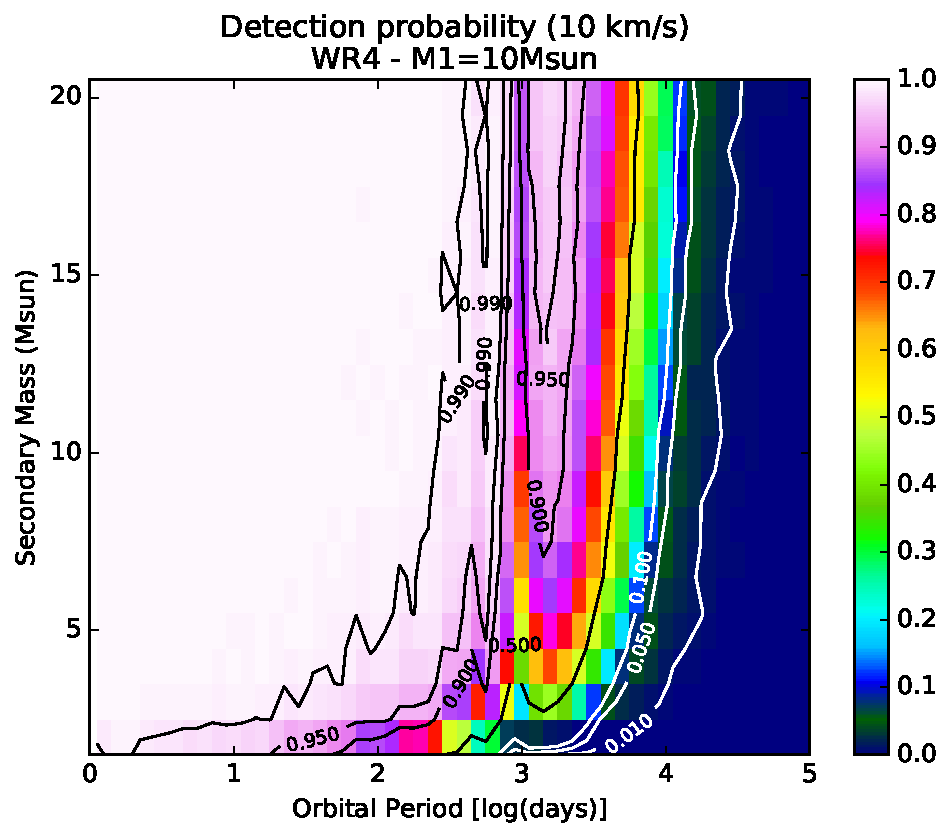
\includegraphics[width=\textwidth]{chapters/appendix3/image/4PM2_thres10_MAR31.pdf}
    \end{minipage}\hfill
    \begin{minipage}{0.49\textwidth}
    \centering
    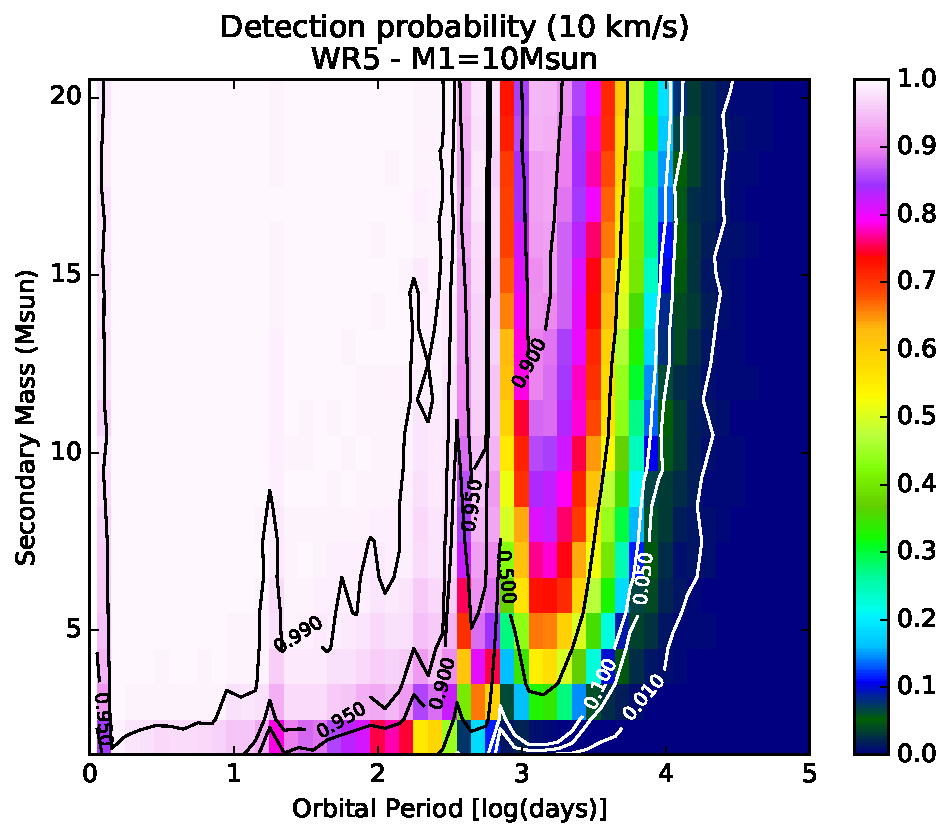
\includegraphics[width=\textwidth]{chapters/appendix3/image/5PM2_thres10_MAR31.pdf}
    \end{minipage}
    \begin{minipage}{0.49\textwidth}
    \centering
    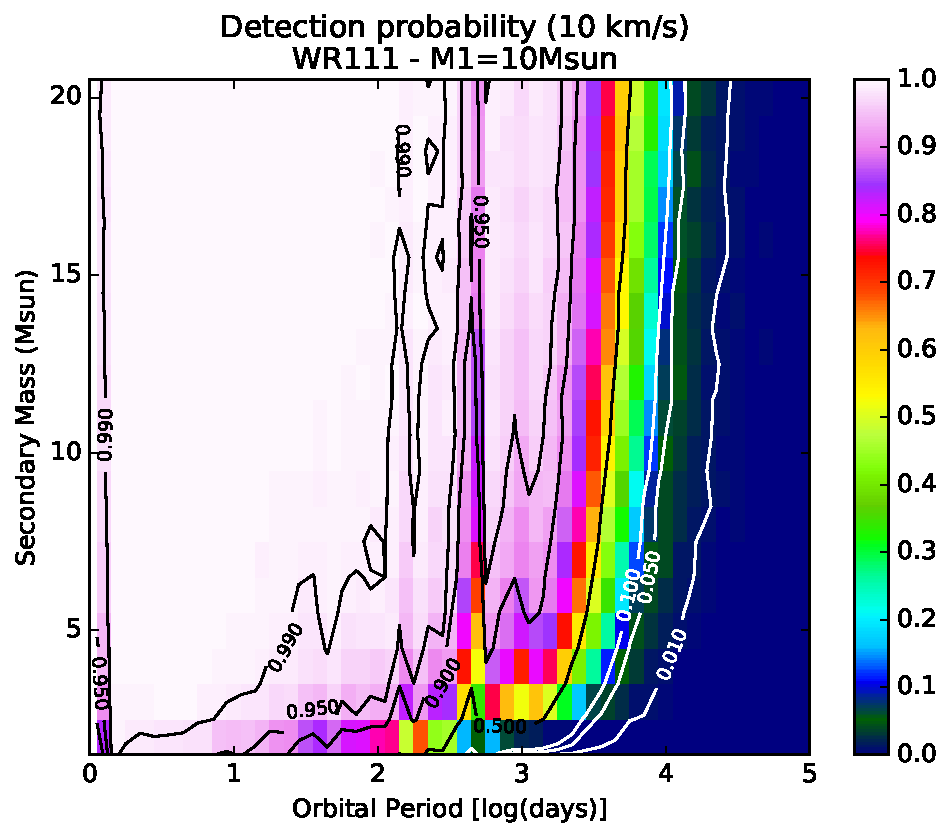
\includegraphics[width=\textwidth]{chapters/appendix3/image/111PM2_thres10_MAR31.pdf}
    \end{minipage}
    \begin{minipage}{0.49\textwidth}
    \centering
    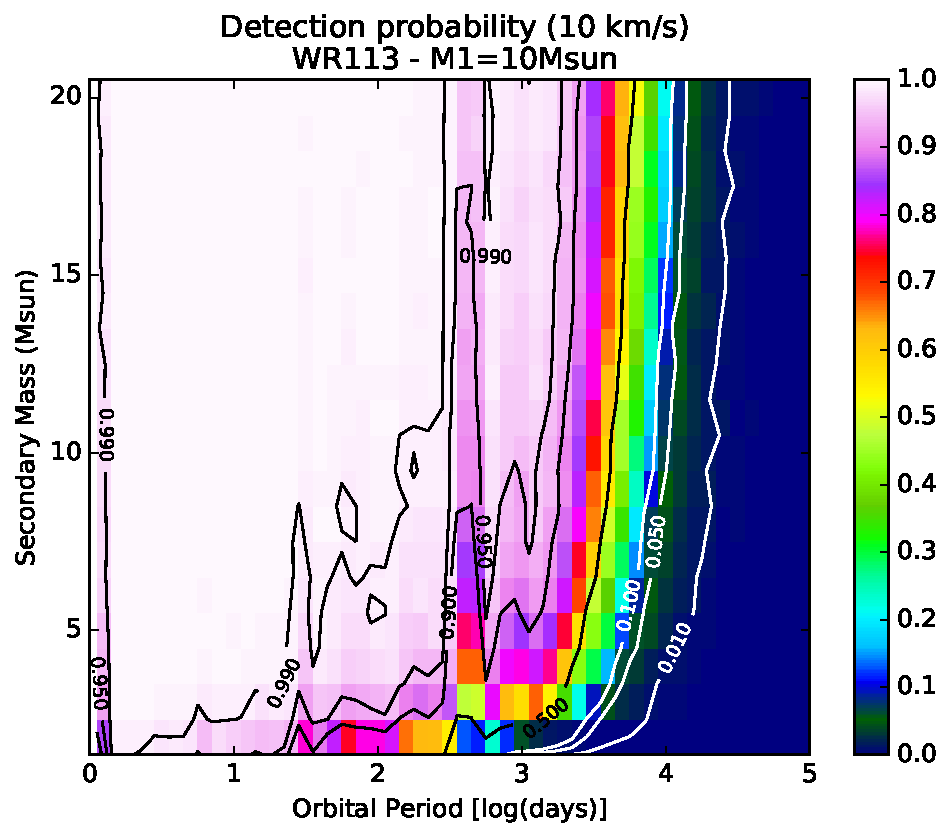
\includegraphics[width=\textwidth]{chapters/appendix3/image/113PM2_thres10_MAR31.pdf}
    \end{minipage}
    \begin{minipage}{0.49\textwidth}
    \centering
    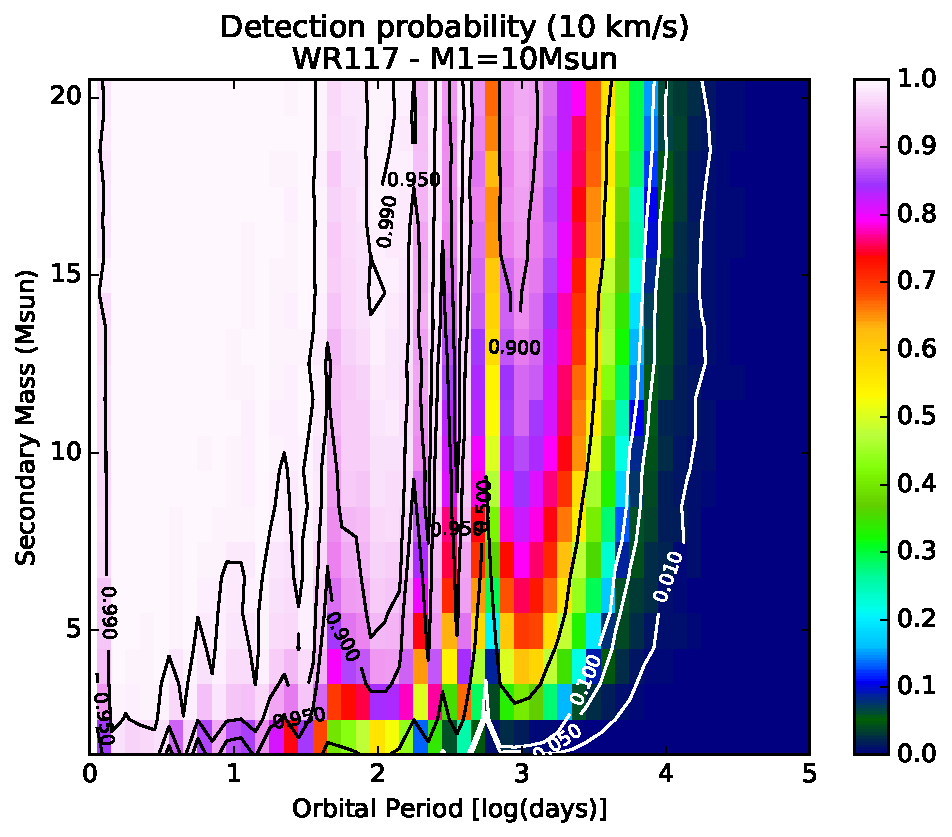
\includegraphics[width=\textwidth]{chapters/appendix3/image/117PM2_thres10_MAR31.pdf}
    \end{minipage}
    \begin{minipage}{0.49\textwidth}
    \centering
    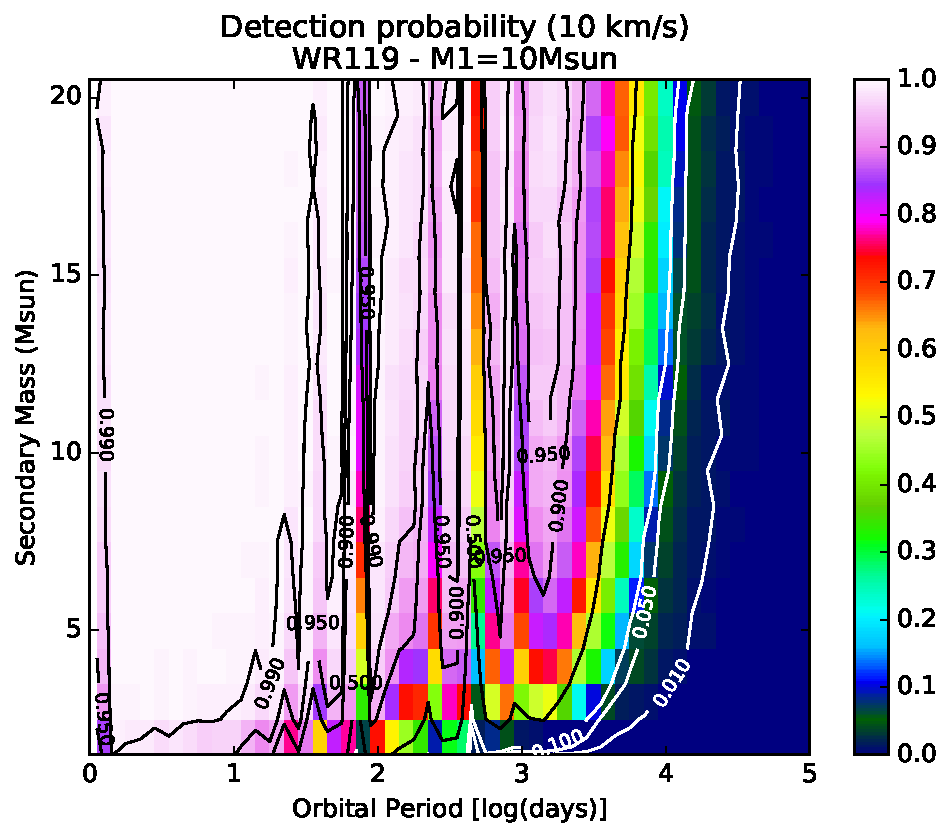
\includegraphics[width=\textwidth]{chapters/appendix3/image/119PM2_thres10_MAR31.pdf}
    \end{minipage}
    \caption{Binary detection probability of the observational campaign for the various stars in our sample, adopting a minimum RV variability threshold of 10~\kms}
    \label{f:Pdetect1}
\end{figure*}
\newpage
\begin{figure*}[h!]
    \centering
    \begin{minipage}{0.49\textwidth}
    \centering
    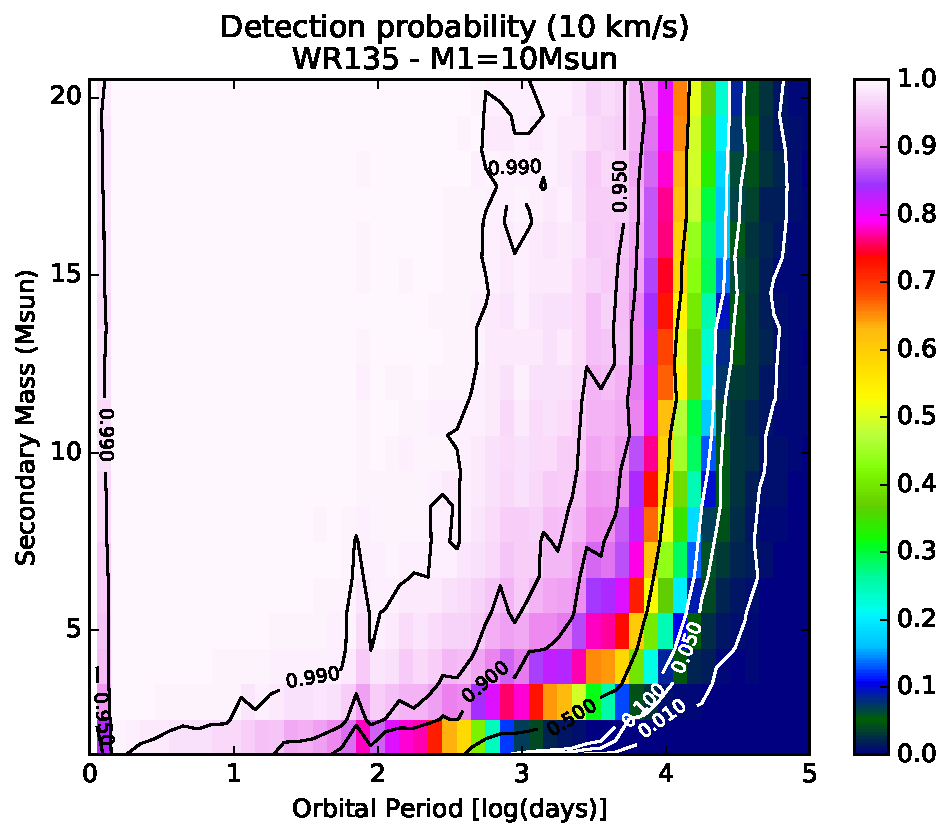
\includegraphics[width=\textwidth]{chapters/appendix3/image/135PM2_thres10_MAR31.pdf}
    \end{minipage}\hfill
    \begin{minipage}{0.49\textwidth}
    \centering
    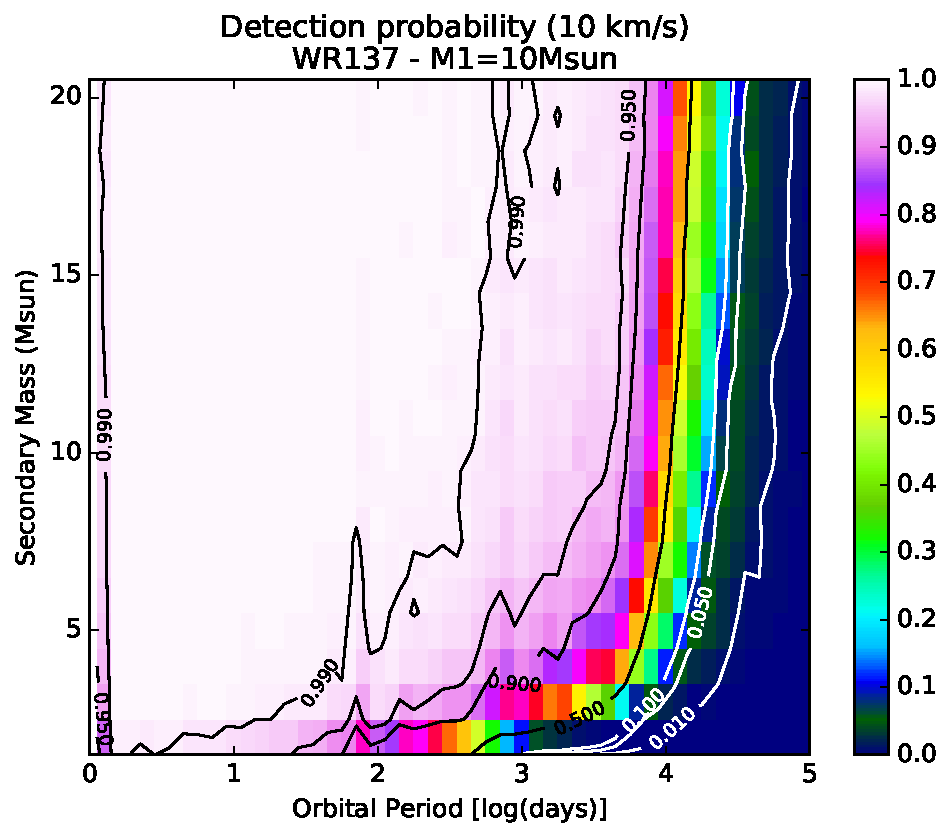
\includegraphics[width=\textwidth]{chapters/appendix3/image/137PM2_thres10_MAR31.pdf}
    \end{minipage}
    \begin{minipage}{0.49\textwidth}
    \centering
    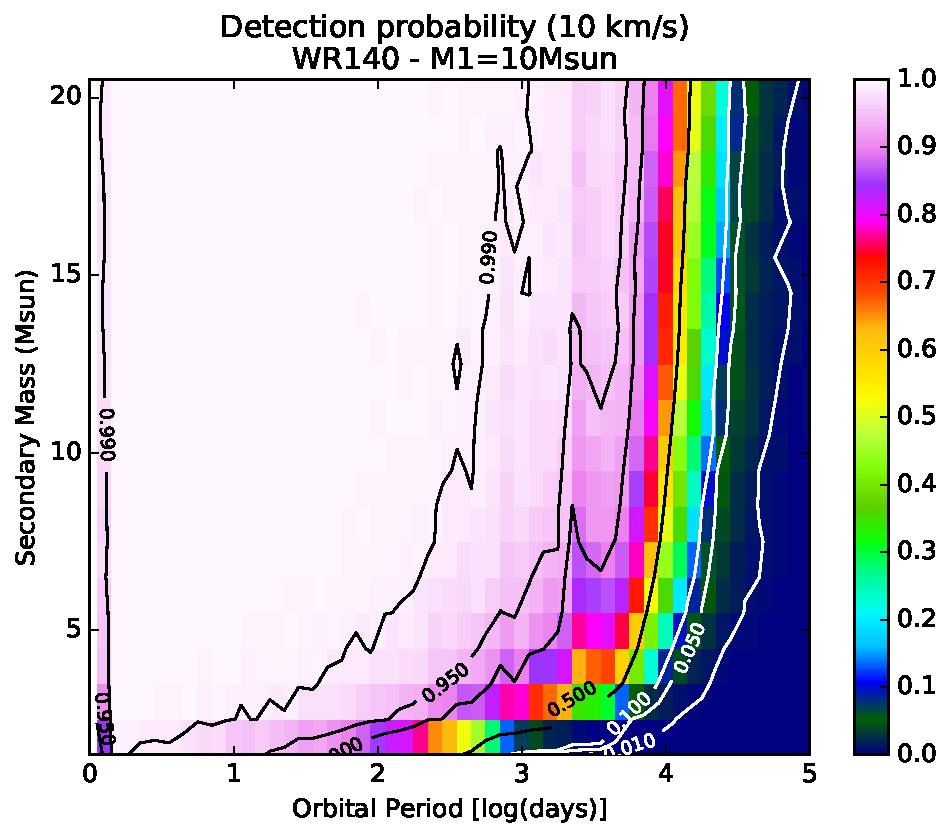
\includegraphics[width=\textwidth]{chapters/appendix3/image/140PM2_thres10_MAR31.pdf}
    \end{minipage}
    \begin{minipage}{0.49\textwidth}
    \centering
    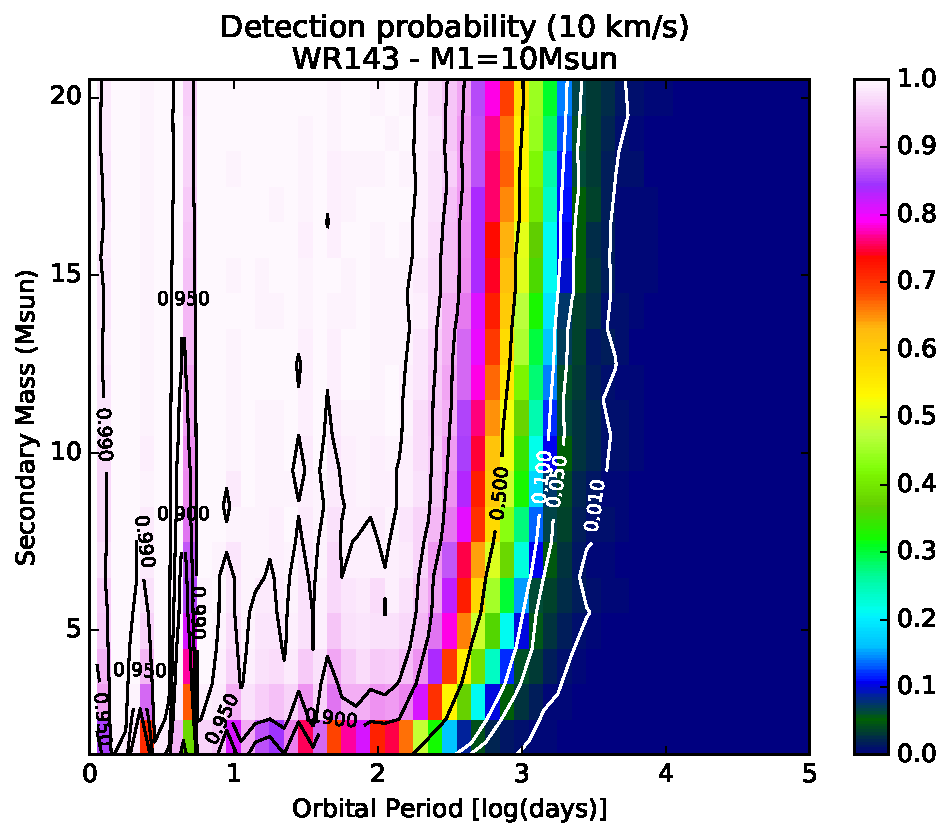
\includegraphics[width=\textwidth]{chapters/appendix3/image/143PM2_thres10_MAR31.pdf}
    \end{minipage}
    \begin{minipage}{0.49\textwidth}
    \centering
    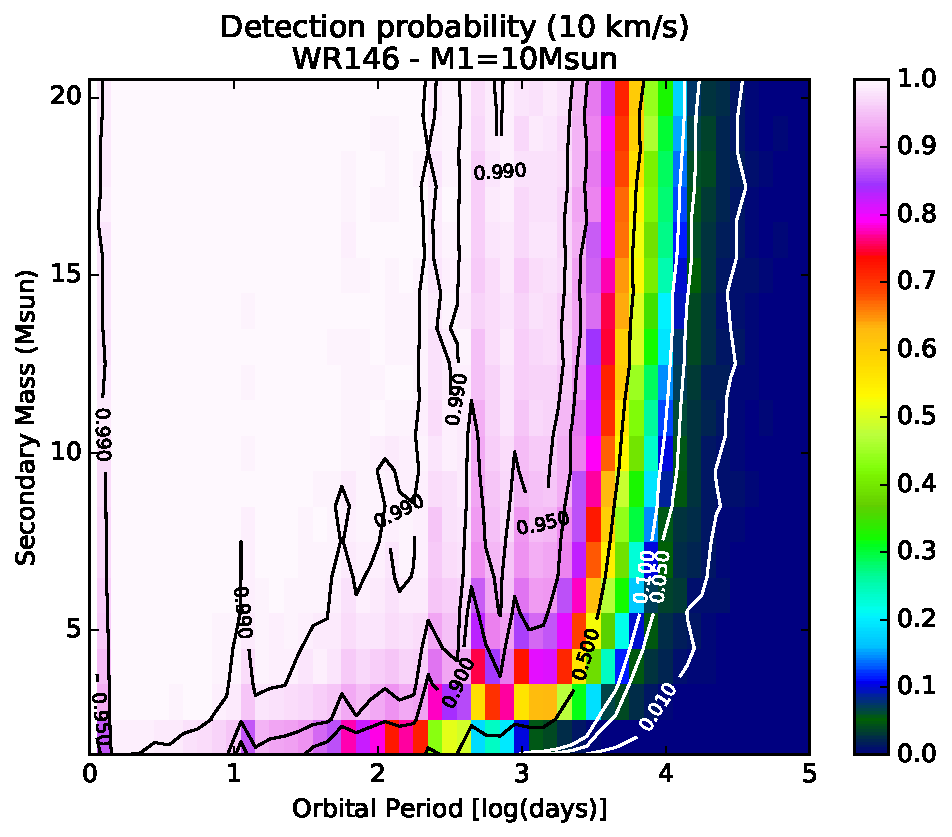
\includegraphics[width=\textwidth]{chapters/appendix3/image/146PM2_thres10_MAR31.pdf}
    \end{minipage}
    \begin{minipage}{0.49\textwidth}
    \centering
    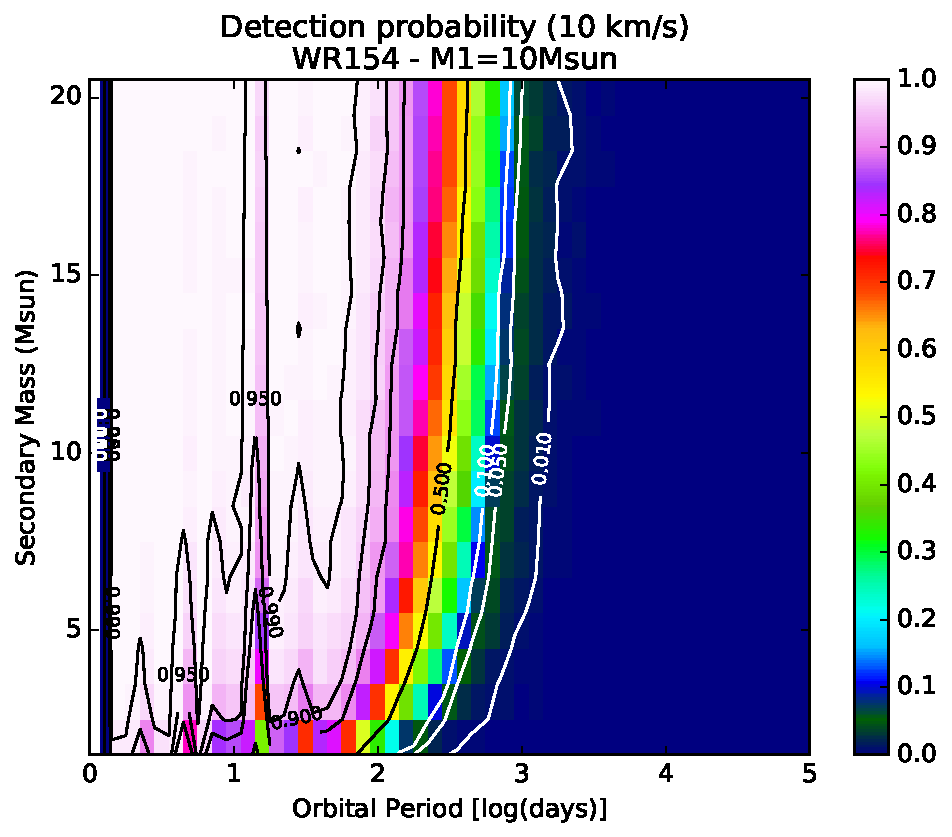
\includegraphics[width=\textwidth]{chapters/appendix3/image/154PM2_thres10_MAR31.pdf}
    \end{minipage}
    \caption{Binary detection probability of the observational campaign for the various stars in our sample, adopting a minimum RV variability threshold of 10~\kms}
    \label{f:Pdetect2}
\end{figure*}

 